\section{Color-Based Mesh Cues}
\label{sec:colormesh}

Since we do not deal with overlapping and highly cluttered background, the segmentation can be done easily by using the color information of the rgb image. The initial segmentation on the leaf is done by using the K-means cluster on the �a� and �b� channels of the Lab color space. It is found that the �a� and �b� channels contain much better information about the green pigments of the leaf. Using only three clusters on these two channels in the k-means clustering, it is able to give a rough mask of where the leaf regions are. But for an accurate mesh fitting, it is required to find the leaf shape by following the edges of the shape boundaries as closely as possible. It is well known in the literature that superpixels ~\cite{achanta2012slic} can split image into multiple homogenous regions and adhere shape boundaries very closely. We use the simple linear iterative clustering (SLIC) superpixels to form superpixels on the entire image. It is found that though SLIC superpixels form an oversegmentation of the image, they are found to adhere very closely to the leaf boundaries. To detect whether each superpixel belongs to the leaf pigments or not, the initial batch of superpixels are selected by computing the centroid of each of them and checking whether it falls within the initial mask developed by K-means cluster. Any non leaf superpixels that are chosen in the first selection are then filtered out by thresholding on the ratio of 'a' and 'b' channels of the Lab color space. The selected superpixels are then merged to create the segmented plant/leaf segment.

We build line segment based on boundary pixels of the segmented plant/leaf boundaries. Since plant leaves are clumped together in a single structure, it is possible to get closed boundary on the entire segmented image of the plant. We then perform a polygonal approximation motivated by the merging technique ~\cite{Leu1988231} process on the boundary by approximating straight lines with a maximum deviation of one pixels from pixels in the original boundary ~\cite{KovesiMATLABCode}. The two end points of the approximated lines are saved as vertices that join an edge of the polygon.

Having obtained the polygonal approximation of the plant leaf boundaries, we then sample points with a uniform spacing of $\ell$ pixels on each side of the polygon. Uniform grid of points with a spacing of $r$ are also created in the entire image, and the grid points which fall within or on the mask structure are only selected. Points falling within $\ell \leq r$ are removed from the set of selected grid points. Both the selected grid points and the sampled points on the boundary are then used to create a delaunay triangulation on the plant mask.The slivers of triangular facets that lie outside the polygonal shape are removed by seeking whether the midpoints of the line fall within the polygonal shape or not.The final meshes on a typical rgb plant image looks like in Figure~\ref{fig:mesh}:

\begin{figure}[!t]
  \vspace{-20pt}
  \centering
  % Requires \usepackage{graphicx}
  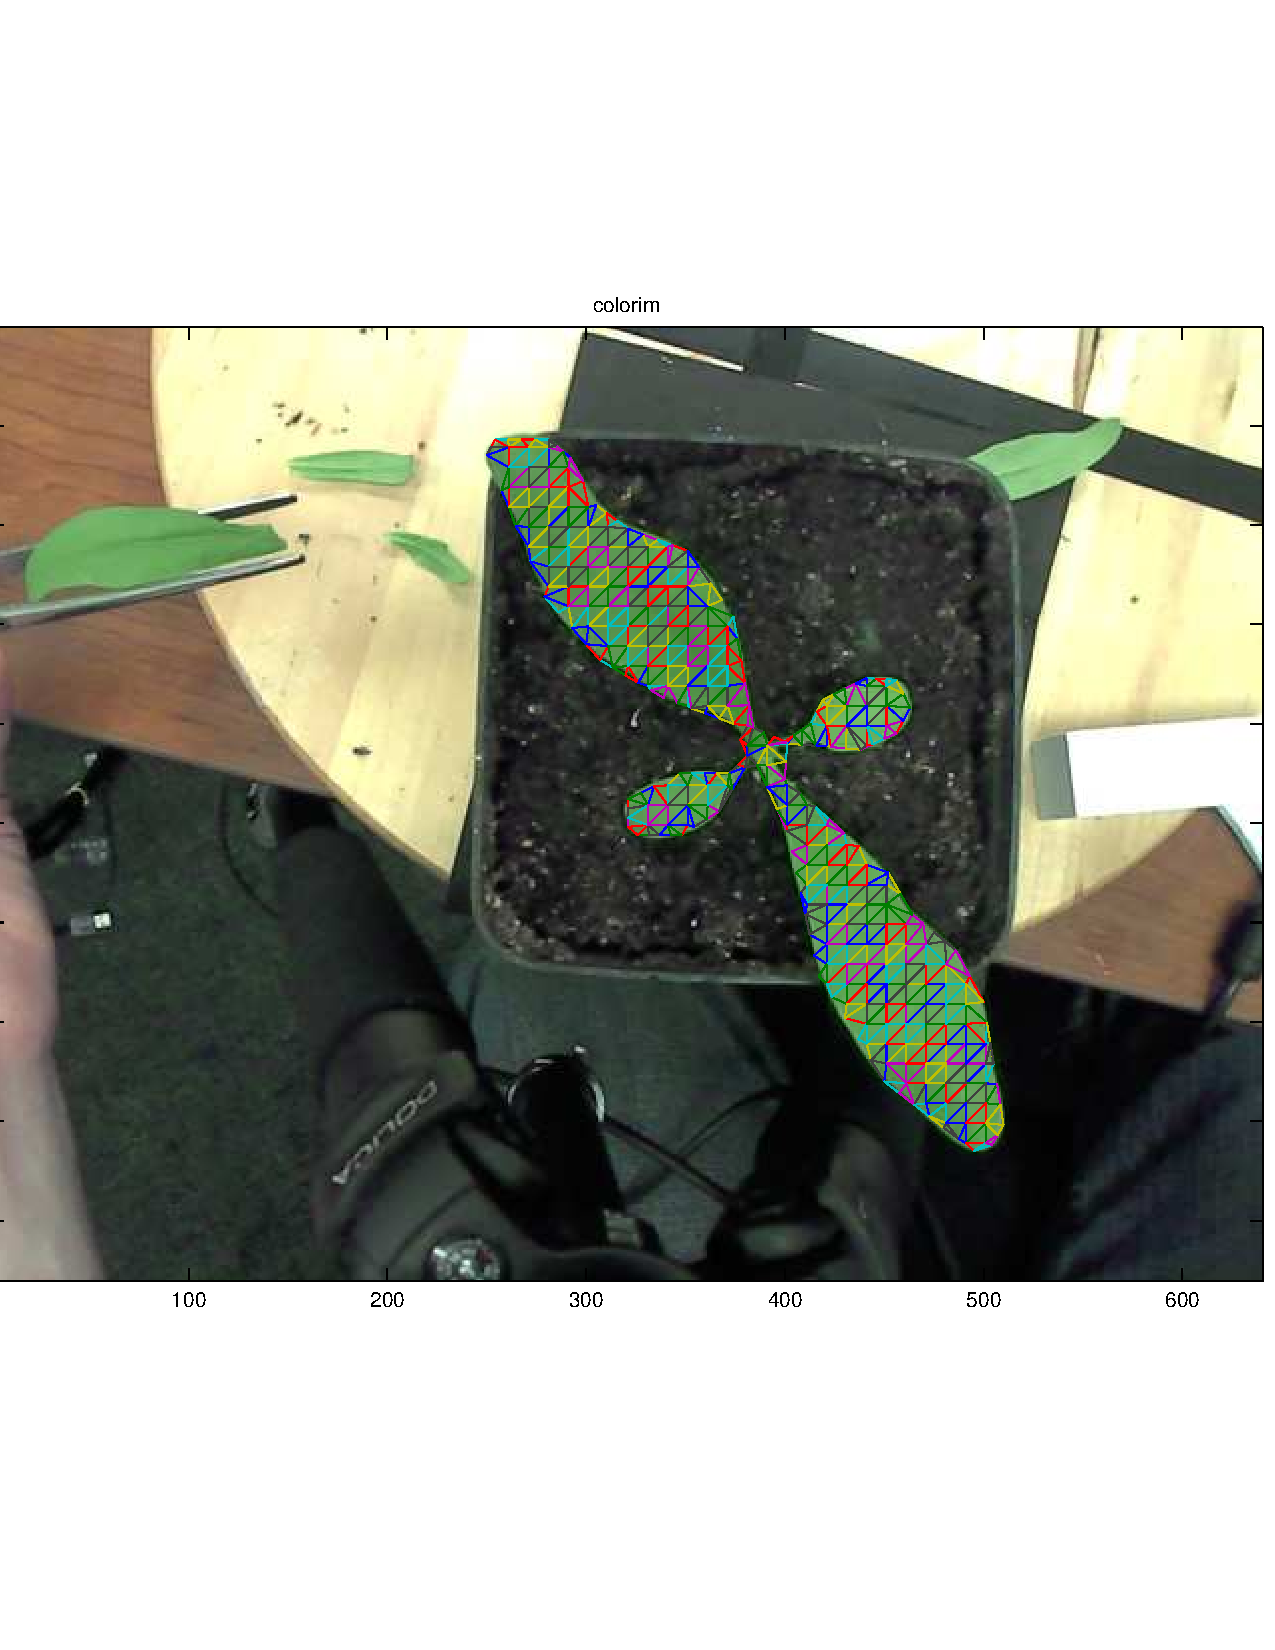
\includegraphics[trim=150 180 120 120,clip,width=0.6\linewidth]{Figures/meshonplant}\\
  \caption{Mesh Distribution on the RGB Plant Imagery}\label{fig:mesh}
\end{figure}

